% !TeX root = ../SDonchezThesis.tex

\chapter{Proposed System Architecture}\label{ch:systemArchitecture}

\section{Proposed Design}\label{subsec:Proposal}
The author proposes modifying the implementation proposed by the authors of \cite{bag_cryptographically_2020}, as outlined in Chapter \ref{ch:relatedWork} to eliminate the need for trust in the CSP, along with eliminating the duplication of the AES IP. To achieve this goal, the author proposes the implementation of an attestably secured partition within the PFPGA fabric, which contains both the KAC and AES engines. By isolating both of these components in an attestably secure partition, the CSP no longer has access to the decrypted symmetric key, preventing them from decrypting the bitstream and gaining access to the IP contained therein. Meanwhile, the presence of the single AES IP in this secured partition eliminates the need for identical engines on each partition, which increases available space and also offers flexibility with regards to VFPGA provisioning, as the only fixed limit remaining is the number of VFPGA device IDs allocated by the FPGA Vendor for the device. This number can simply be made arbitrarily large relative to the realistic number of simultaneous tenants that the device can support, such that the CSP is effectively free to divide the PFPGA as they see fit.

% The presence of a secure partition for decryption operations is useless without the ability to securely transport the decrypted data from said partition to the VFPGA in question. The use of the Hard Processor System (HPS), and specifically a Trusted Execution Environment (TEE) implemented therein, could conceivably facilitate the secure transfer of this information between regions of the FPGA without transiting the unsecured outer region of the programable logic. However, implementation of direct connections between partitions and the HPS such as this necessitates will require further investigation, as the mechanics of such an operation are not currently understood by the author. Alternatively, the use of direct memory access could be a route to secure transfer, although assurance must exist to prevent malicious access to the memory regions in question.

The presence of a secure partition for decryption operations is useless without the ability to securely transport the decrypted data from said partition to the VFPGA in question. Such a task is made far more difficult by the fact that the PFPGA only has a single set of physical connections to the physical memory, which must be commonly utilized by all of the partitions. This requires one of several strategies to ensure data integrity. One option would be for the CSP to allocate dedicated Block RAM to each partition and allow access to it only from the decryption partitions and the given tenant partition. However, such a solution would likely be prohibitively expensive, and would still require the data to traverse an untrusted region of the FPGA at some point.

As an alternative, this paper proposes the use of a trusted (provided by either the FPGA vendor or a trusted third party) top level bitstream, incorporating memory isolation technology contained in the trusted top level bitstream in order to prevent co-tenants from accessing each others' data. This memory isolation logic, for shared resources such as the decryption partitions, could be dynamically configured within the HPS. Such an architecture is captured in Figure \ref{fig:topLevelDesign}, where the memory isolation logic is shown implemented at each partition boundary.

\begin{figure}
  \centering
  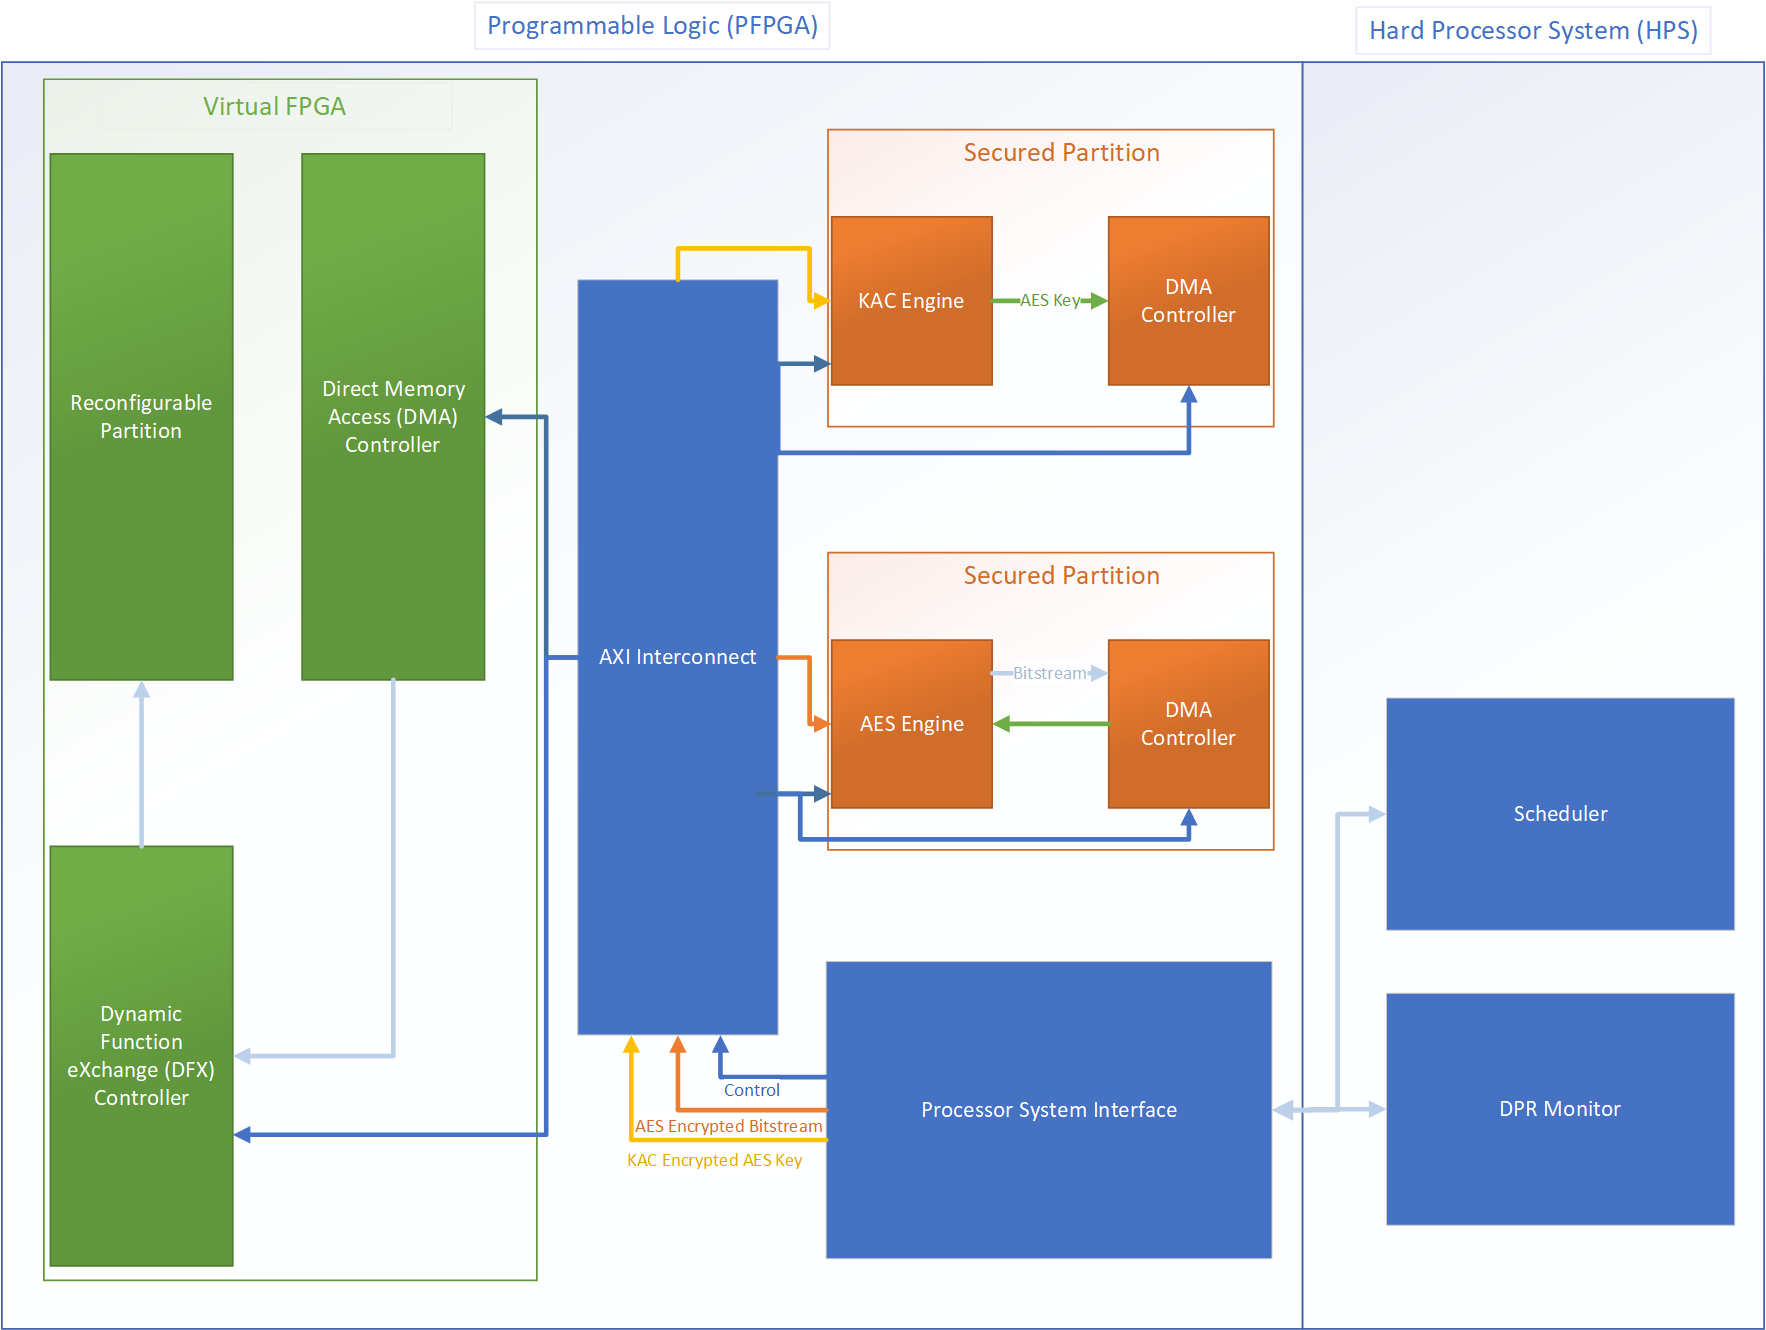
\includegraphics[width=0.8\textwidth]{ConceptDiagramSimplified.png}
  \caption{System Architecture Concept Diagram}
  \label{fig:topLevelDesign}
\end{figure}

The use of the HPS to facilitate such a transfer has additional advantages, as it is conceivable on larger devices that multiple such partitions could be desired to facilitate simultaneous tenant reprogramming. In either case, the use of the HPS to schedule access to the secured partition(s) could similarly prove to be a useful design component.

\section{Architecture Implementation Tasks}\label{subsec:Obj}
The above implementation requires a number of discrete objectives be completed and integrated into a comprehensive design. Those objectives are described below.

\begin{itemize}
  \item Obtain or design the AES and KAC cores for the secured partition.
    \begin{itemize}  
      \item Ideally these cores should be pipelined for efficiency
    \end{itemize}
  \item Investigate direct communication between partition and HPS (without untrusted transit)
  \item Investigate use of DMA to facilitate secure communication between partitions securely
  \item Design and Implement scheduling algorithm to allocate decryption partition to tenants
    \begin{itemize}
      \item With multiple AES cores, it may make sense to share a single KAC engine if a secured link between them can be guaranteed (the KAC has to decrypt a single key of trivial size, whereas the AES engine is in much higher demand due to need to decrypt entire bitstream)
    \end{itemize}
  \item Implement attestably secure partition and provide mechanism for attestation and verification
  \item Implement Trusted Execution Environment (within HPS for purposes of supervision and security monitoring)
  \item Implement data routing and verification logic within TEE
  \end{itemize}

The remaining chapters of this work (with the obvious exception of the conclusion) explore the design and implementation of several of these objectives. Although they do not provide a robust implementation of the entire proposed architecture (as the scope of that work was deemed too large for the given time constraints), they represent the elaboration of those features which were considered both substantial and novel, as well as closely related to the Programmable Logic portion of the system. As was briefly mentioned in Section \ref{sec:organization}, they are organized as follows.

Chapter \ref{ch:edfScheduling} addresses the fourth objective above, the implementation of a real-time, aperiodic scheduling algorithm to enable the efficient allocation of decryption engines to various tenants as they attempt to program their partition. This is critical to breaking the one to one relationship between partitions and decryption engines, which drastically limits the scalability of existing systems. The algorithm proposed in Chapter \ref{ch:edfScheduling} enables multiple partitions to share a single decryption engine, while ensuring that any resource contention is decided equitably on the basis of timing constraints.

Chapter \ref{ch:keyAggregateCryptography} expands on this work by providing a discussion on the implementation of a Key-Aggregate Cryptosystem (KAC), which has been proposed in at least one current architecture found in literature. The use of a KAC enables the tenant to be assured of the limited scope in which their bitstream can be decrypted, by localizing it to a specific hardware device while enabling encryption operations to utilize a single shared key. Although this work does not specifically develop a KAC implementation itself (as such an effort would require mathematical experience outside the scope of this research), it instead provides a rigorous discussion of theoretical operation of such an implementation, of which only few instances exist in literature. It also provides a detailed analysis of the application of such an engine to this architecture, and to the cloud FPGA lifecycle as a whole.

Finally, Chapter \ref{ch:dmaProtection} concludes the body of this work by discussing objectives two and three in the list above - the secure transit of decrypted data between regions of the FPGA. It takes a two factor approach to this - one designed to protect against malicious co-tenants, and one designed to provide assurances as to the integrity of the CSP's supervisory logic. To address the latter, Chapter \ref{ch:dmaProtection} proposes a FPGA-vendor provided supervisory bitstream, with attestability integrated for user assurance. The body of the chapter, meanwhile, discusses the more difficult problem of tenant isolation, utilizing Xilinx logic to isolate each partition from the outside world through the use of Memory Isolation IP.
